\section{Instruction Execution Cycle}

\subsection{Terminologies and Basic Information}

Terminologies:
\begin{itemize}
    \item \textbf{Byte}: 8 bits, smallest addressable unit of memory.
    \item \textbf{Word}: Unit of organisation of memory, varies from system to system.
        e.g. 32-bit, 64-bit, etc.
    \item \textbf{Register}: Small, fast storage location within the CPU.
    \item \textbf{Word Addressing}: Addresses of memory on a computer that uniquely
        identify a word.
    \item \textbf{Byte Addressing}: Addresses of memory on a computer that uniquely
        identify a byte.
\end{itemize}

Registers inside a CPU:
\begin{itemize}
    \item \textbf{PC (Program Counter)}: Holds the address of the next instruction
        to be fetched.
    \item \textbf{IR (Instruction Register)}: Holds the current instruction.
    \item \textbf{MAR (Memory Address Register)}: Holds the address of the memory
        location to be accessed.
    \item \textbf{MBR (Memory Buffer Register)}: Holds the data to be written to
        or read from memory. (Also, MDR)
    \item \textbf{I/O AR} and \textbf{I/O BR}: Similar to MAR and MBR, but for I/O
        operations.
\end{itemize}
Data are transferred through system bus. The source register put the data on the bus,
then the destination register pulls the data from it. At any given time, only one
data transfer can be performed on one bus.

\subsection{Instruction Execution Cycle}

\begin{remark}
    This note assumes the computer uses 32-bit word.
\end{remark}

\begin{figure}[H]
    \centering
    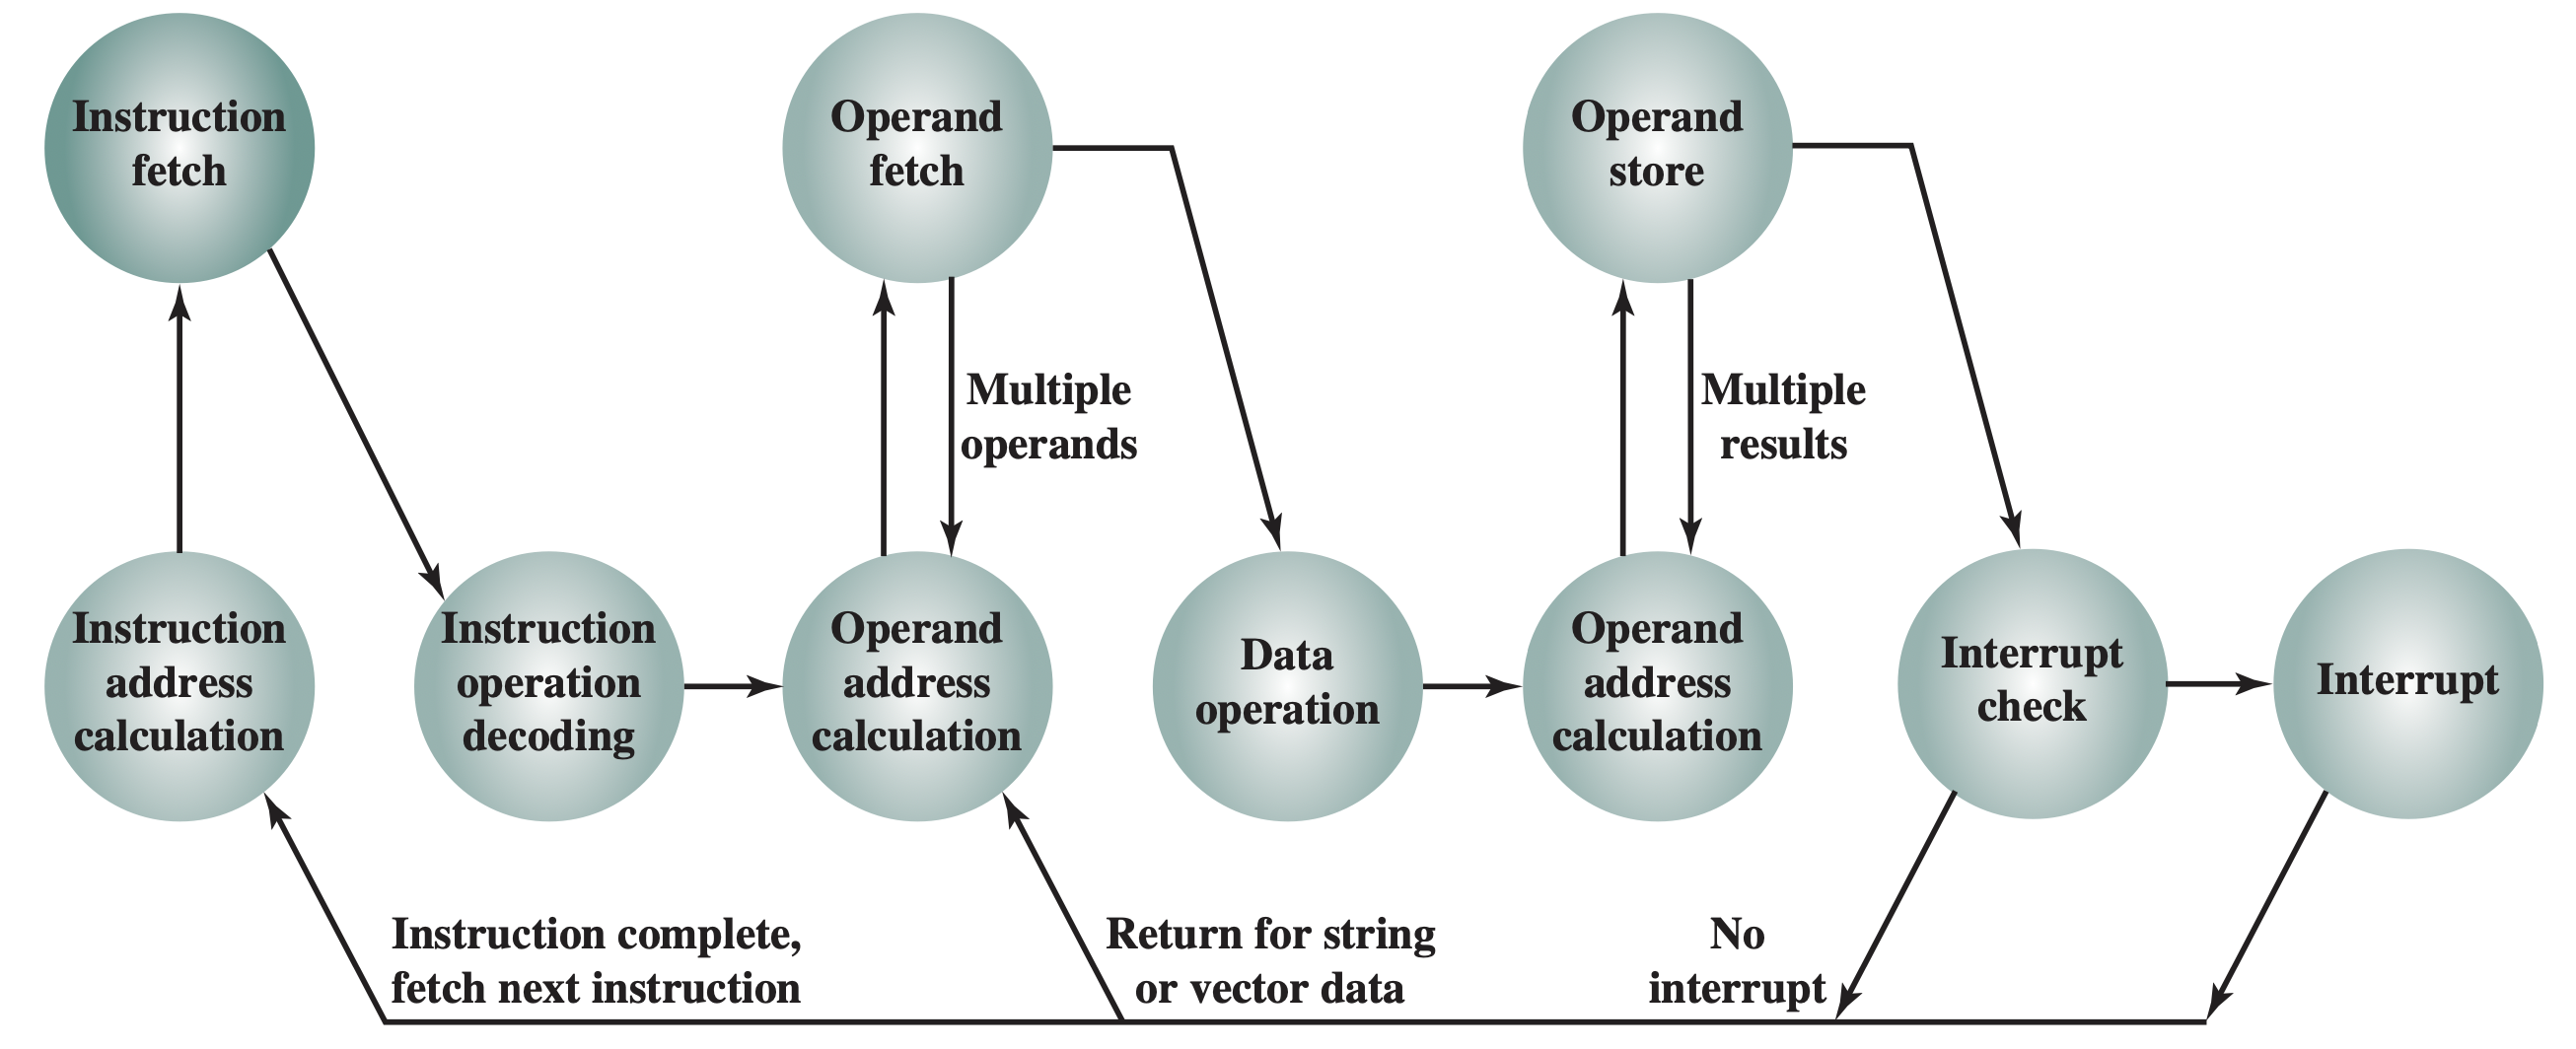
\includegraphics[width=0.85\textwidth]{chaps/instruction-execution-cycle/instruction-cycle-interrupts.png}
    \caption{Instruction Execution Cycle with Interrupts Handling}
\end{figure}

\subsubsection{Instruction Format}

An instruction can be one-word or multi-word. A typical form of instruction may have the
format of:
\begin{table}[H]
    \centering
    \begin{tabular}{cccc}
        Byte 0                       & Byte 1                                & Byte 2                                & Byte 3                                   \\ \hline
        \multicolumn{1}{|c|}{Opcode} & \multicolumn{1}{c|}{Source Operand 1} & \multicolumn{1}{c|}{Source Operand 2} & \multicolumn{1}{c|}{Destination Operand} \\ \hline
    \end{tabular}
\end{table}
where opcode stands for operation code, for example, \texttt{ADD (0x00)}, \texttt{SUB (0x01)},
\texttt{AND (0x02)}, \texttt{OR (0x03)}, \texttt{NOT (0x04)} etc.

\begin{enumerate}

\item \textbf{Arithmetic and Logical Operations}:

Consider this operation: \texttt{ADD R1, R2, R3} (or in pseudocode, \texttt{R3 = R1 + R2}),
the instruction is represented as \texttt{0x00010203}. Since \texttt{ADD} requires two source
operands and one destination operand, all fields are used.

Consider \texttt{NOT R1, R2} (or in pseudocode, \texttt{R2 = NOT R1}), the instruction is
represented as \texttt{0x04010002}. Since \texttt{NOT} uses only one source operand, the
second source operand is set as \texttt{0x00}.

\item \textbf{\texttt{LD} and \texttt{ST} Instructions}:

For instructions that uses memory, a two-word instruction is needed as the memory address
cannot fit in the operand. Assume that \texttt{LD (0x06)} and \texttt{ST (0x07)}.
For example, \texttt{LD P1(0x0000003c), R1}, which loads the content of
memory address \texttt{P1} to register \texttt{R1}, the instruction is represented as
\texttt{0x0600ff01 0000003c}. The format is:
\begin{table}[H]
    \centering
    \begin{tabular}{ccccclll}
    Byte 0                       & Byte 1                                     & Byte 2                                      & Byte 3                                   & Byte 4    & Byte 5    & Byte 6    & Byte 7   \\ \hline
    \multicolumn{1}{|c|}{Opcode (\texttt{LOAD})} & \multicolumn{1}{c|}{Source (\texttt{0x00})} & \multicolumn{1}{c|}{Addressing Model (\texttt{0xff})} & \multicolumn{1}{c|}{Destination} & \multicolumn{4}{c|}{Memory Address} \\ \hline
    \multicolumn{4}{c}{Word 0}                                                                                                                                         & \multicolumn{4}{c}{Word 1}                  
    \end{tabular}
\end{table}

\begin{remark}
    For simplicity, there is only one addressing model (\texttt{0xff}) used in this section.
\end{remark}

\item \textbf{Branching Instructions}:

A branching instruction has the following format:
\begin{table}[H]
    \centering
    \begin{tabular}{ccccclll}
    Byte 0                                & Byte 1                              & Byte 2                                         & Byte 3                          & Byte 4     & Byte 5     & Byte 6     & Byte 7    \\ \hline
    \multicolumn{1}{|c|}{Opcode (Branch)} & \multicolumn{1}{c|}{Condition Code} & \multicolumn{1}{c|}{Address/Addressing Model} & \multicolumn{1}{c|}{(not used)} & \multicolumn{4}{c|}{Address of Destination Instruction} \\ \hline
    \multicolumn{4}{c}{Word 0}                                                                                                                                     & \multicolumn{4}{c}{Word 1}                      
    \end{tabular}
\end{table}

Examples of condition codes are:
\begin{table}[H]
    \centering
    \begin{tabular}{|c|c|l|}
    \hline
    \textbf{Instruction} & \textbf{Condition Code} & \textbf{Meaning} \\ \hline
    \texttt{BR} & \texttt{0x00} & Unconditional branch \\ \hline
    \texttt{BZ} & \texttt{0x01} & Branch if zero \\ \hline
    \texttt{BNZ} & \texttt{0x02} & Branch if not zero \\ \hline
    \end{tabular}
\end{table}
By saying ``zero'', it means to check the zero flag of the ALU to determine if the previous
operation resulted in zero. Other flags may also be used.

\begin{example}
    Consider this code (on the right side is the machine code in hexadecimal):
    \begin{minted}[style=friendly]{asm}
        LD  P2, R2      ;                       0000: 0600ff02 00000034
        LD  P1, R1      ;                       0008: 0600ff01 00000030
        LD  P3, R3      ;                       0010: 0600ff03 00000038
        MOV R2, R4      ;                       0018: 05020004
    L:  ADD R2, R3, R2  ; Increment R2 by 1     001C: 00020302
        SUB R1, R2, R4  ; R4 = R1 - R2          0020: 01010204
        BNZ L           ; If R4 != 0, go to L   0024: 0802ff00 0000001C
        HLT             ;                       002C: 09000000 
    P1: .WORD 5         ;                       0030: 00000005
    P2: .WORD 0         ;                       0034: 00000000
    P3: .WORD 1         ;                       0038: 00000001
    P:  .WORD           ;                       003C: 00000000
    \end{minted}
    The \texttt{BNZ} instruction is used to create a loop that increments \texttt{R2} by 1
    until \texttt{R1 - R2} is zero. The program halts when the condition is met.
\end{example}

\item \textbf{Halt Instruction}:

The \texttt{HLT} instruction is used to halt the program. It does not use any operands
and those fields are set to \texttt{0x00}.

\end{enumerate}

\subsubsection{Instruction Fetch}

Address to the next instruction is stored in PC register, which is incremented automatically
during execution. For a two-word instruction, the first word is fetched first, then PC
is incremented by 1 word to point to the second word. Then the second word is fetched,
and PC is incremented again to point to the next instruction.

Note that PC is will be changed when branching happens.

This process is called Instruction Address Calculation (IAC).

During IF, the following data transfer happens:
\begin{align*}
    \text{MAR} &\leftarrow \text{PC} \\
    \text{PC} &\leftarrow \text{PC} + 1 \\
    \text{MBR} &\leftarrow \text{Memory}[\text{MAR}]
\end{align*}

\subsubsection{Instruction Decode}

The control unit will decode the instruction and setup the ALU and other components
for appropriate operations (e.g. memory read/write, data transfer, etc.). These actions
are carried out at appropriate times by the control unit.

\subsubsection{Operand Fetch}

If the operands are in registers, data are moved from registers to ALU.

If the operands are in memory, then the instruction would be a two-word instruction.
Note that if PC points to the second word of a two-word instruction, after the above process,
MBR will contain the \textbf{address} of the second word, not the content. Therefore, another
memory read is needed to fetch the content, by:
\begin{align*}
    \text{MAR} &\leftarrow \text{MBR} \\
    \text{MBR} &\leftarrow \text{Memory}[\text{MAR}]
\end{align*}

\subsubsection{Execution}

The ALU performs the operation specified by the instruction. The result is stored in
some temporary register.

\subsubsection{Result Store}

Similar to operand fetch, if the destination is in register, RF write is performed.
If the destination is in memory, then operand address calculation is first performed.
Then the data is written to memory.

\subsubsection{Interrupt Handling}

Interruptions are important as:
\begin{itemize}
    \item They improve efficiency.
    \item When an I/O arrives, it may need immediate attention, or data may be lost.
        e.g. incoming data from a network.
    \item Other programs may also need the CPU's attention. e.g. on a time-sharing system.
\end{itemize}

When interruption is required, I/O device sends a signal to the CPU. The CPU will need to
remember the current state of the program, and then jump to serve the interrupt. The CPU
will then return to the original program and continue execution as if nothing happened.

Interrupt handlers can either be hardware or software.

Interrupt signals are checked at the end of one complete instruction cycle, minimising the
registers that need to be saved/restored. Before each interrupt, the following information
is saved (by pushing to the stack):
\begin{itemize}
    \item Flag register -- to remember the state of the ALU.
    \item PC -- to remember the address of the next instruction.
    \item Modified register files.
    \item The current address of the instruction -- to remember where the program was
        interrupted, while the address of the interruption program is loaded to PC.
\end{itemize}
Other registers (like MAR, MBR, IOAR, etc.) are not saved as they are only meaningful
during the current instruction cycle.